\part{Entwicklerhandbuch}

\chapter{Übersicht}
\section{Technologien}

\section{Systemvoraussetzungen}

\section{Build-Prozess}


\chapter{Software-Entwurf}
\section{Komponentenstruktur}

\section{Design Pattern}

\section{Klassendiagramm}


\chapter{Implementierung}
\section{Logik und Algorithmus}
\todo{hier muss erklärt werden wie der Algorithmus mit den Zählern funktioniert und ggf. warum das O(1) ist}

\section{Benutzerschnittstelle}
\todo{hier muss erklärt werden wie ReactJS funktioniert und warum es die Performance verbessert}
Damit die aktiven Zustände hervorgehoben werden können, müssen sie eindeutig identifizierbar sein. Dafür wurden die Elemente der Grafik gruppiert und mit IDs versehen, auf die mittels Javascript und dem \acrshort{DOM} zugegriffen werden kann. Abbildung \ref{fig:ZD_id_view} stellt die Identifikatoren dar. Bei der Benennung der IDs wurden folgende Konventionen angwendet:
\begin{itemize}
	\item präfix uml- für alle Bezeichner
	\item Worte durch Bindestriche getrennt
\end{itemize}

\begin{figure}[hbt]
	\centering
	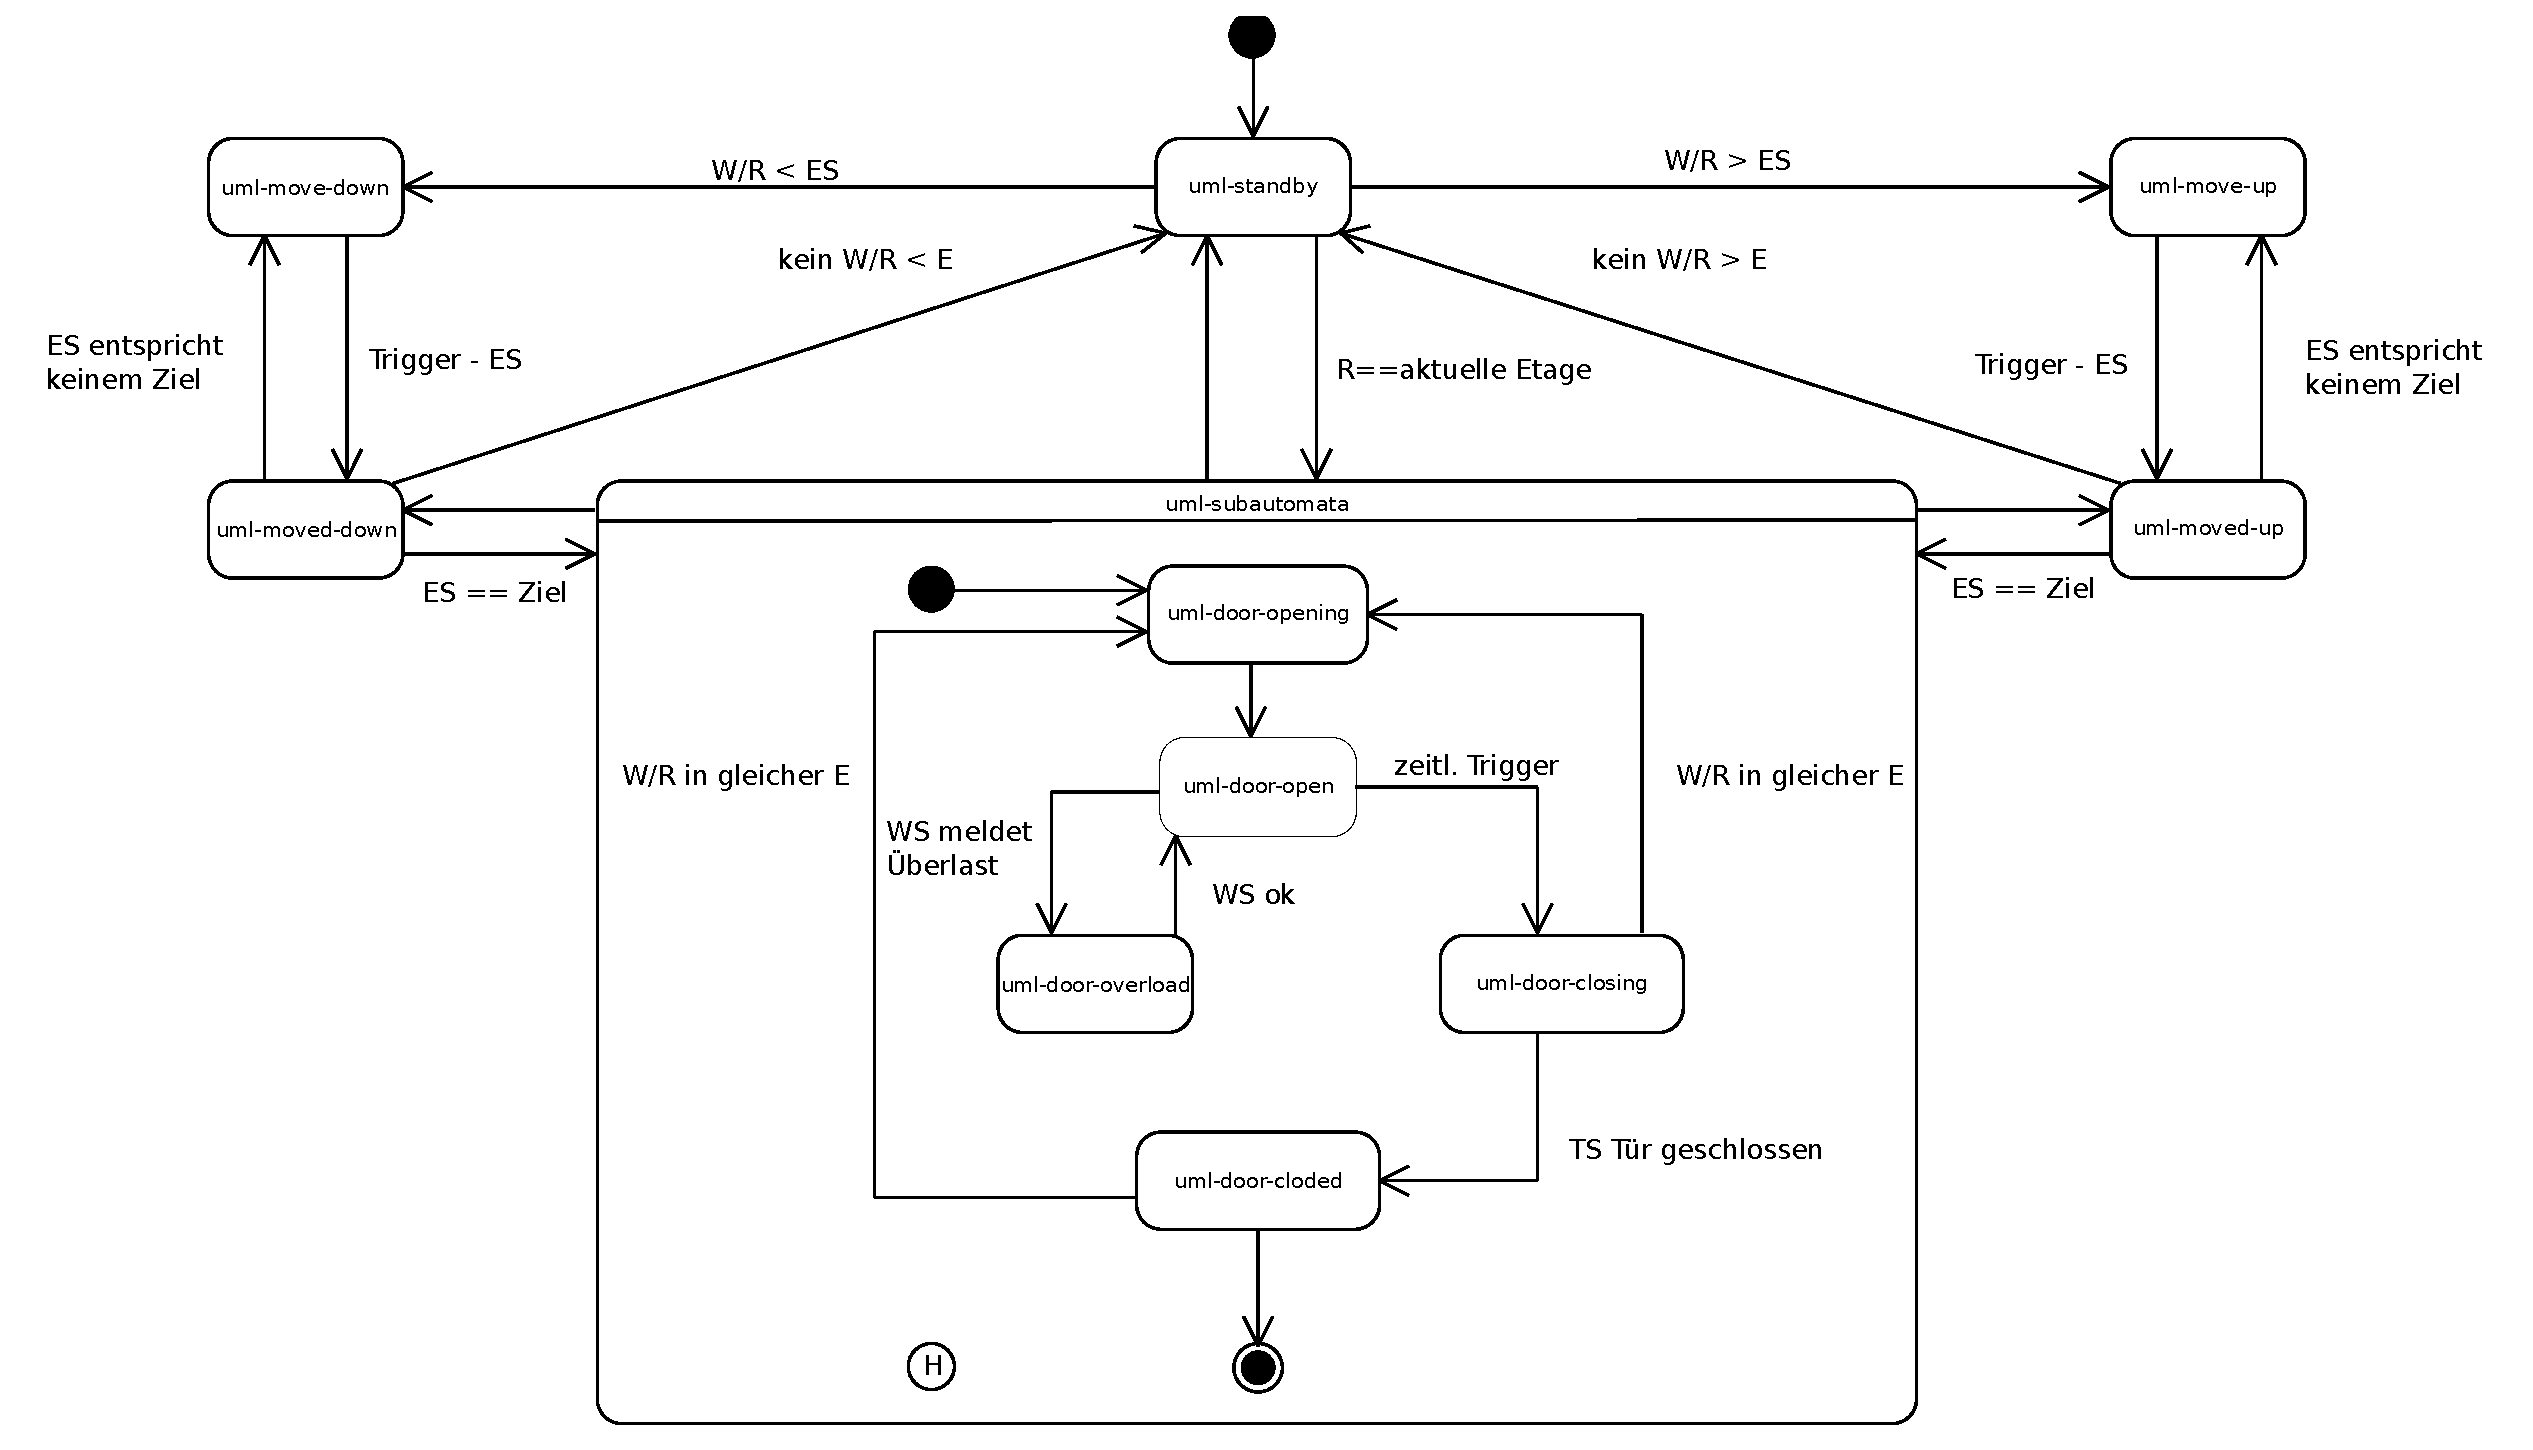
\includegraphics[width=\textwidth]{images/ZDv6_id_view.eps}
	\caption{IDs des Zustandsdiagrammes}%
	\label{fig:ZD_id_view}%
\end{figure}

\section{Erweiterungen}

